\section{Analysis}

From Tab.\,\ref{t:lebensdauer} one can see, that the measurement for the lifetime of muons significantly depends on the fitrange that is used for the analysis. One can also see, that the fits don't give an excellent $\chi^2_{red}$ which is an indicator for an imperfect model with some systematic effect not taken into account. The fits for the decays down are better than the decays up, this might be because the afterpulses play a much less significant role for the decays downwards. From the variation of the lifetime with the fitrange, one can estimate the systematic error by calculating the sample standard deviation ($\sigma_{sys} = \frac{1}{N-1}\sum_{i=1}^N(\tau_i-\bar{\tau})^2 = 0.26$). This yields 
\begin{equation}
	\tau_0 = (2.02\pm0.04_{\text{stat}}\pm0.23_{\text{sys}})\mu\text{s},
\end{equation}
where the statistical error comes from the fit. 

When taking into account the capturing of negative muons by atoms one gets slightly different results, as can be seen in Tab.\ref{t:einfangzeiten}. Firstly one can see, that the $\chi^2_{red}$ is significantly reduced for all the fits, which shows, that the model has been improved by taking the capturing into account. Yet it is still a little bit too high, which hints at other systematic error sources that have not been taken into account. 
From this data we get analogously to before
\begin{equation}
	\tau_0 = (2.28\pm0.05_{\text{stat}}\pm0.22_{\text{sys}})\mu\text{s}
\end{equation}
and
\begin{equation}
	\tau_c = (1.22\pm0.15_{\text{stat}}\pm0.25_{\text{sys}})\mu\text{s}.
\end{equation}
The systematic error from the Parameter f and the scaling factors are negligible compared to the big systematic error from the fit range. Using
\begin{equation}
	G_F^2 = \frac{192\pi^3\hbar}{\tau_0(m_\mu c^2)^5}
\end{equation}
we get
\begin{equation}
	G_F = (1.14 \pm 0.03_{\text{stat}} \pm 0.11_{\text{sys}})\cdot 10^{-5}\frac{1}{\text{GeV}^2}
\end{equation}

From the polarisation measurement we get a Larmor frequency of $\omega_L =3.0\pm0.1_{\text{stat}}$MHz or $\omega_L = 2.74\pm0.31_{\text{stat}}$MHz depending on the fitrange. There has not been enough analysis done to systematically give a systematic error, it is estimated to be $\sigma_{sys}\approx0.3$MHz, yielding
\begin{equation}
	\omega_L =2.9\pm0.2_{\text{stat}}\pm0.3_{\text{sys}}\text{MHz}
\end{equation}
Where the systematic error sources that have been discussed above should play a role. Also not subtracting the after pulses could mess with the results. 
Using
\begin{equation}
	\mu_{\mu}^{\text{Bohr}} = \frac{\hbar\omega_L}{gB} 
\end{equation}
we get
\begin{equation}
	\mu_{\mu}^{\text{Bohr}} = (3.82\pm0.26_{\text{stat}}\pm0.39_{\text{sys}})
\end{equation}

\begin{figure}[H]
    \centering
    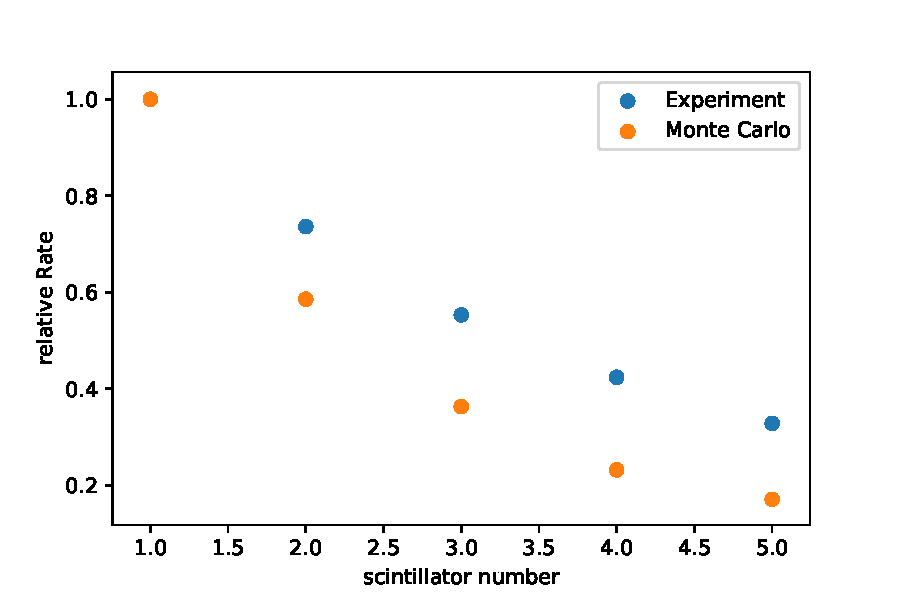
\includegraphics[width=0.5\textwidth]{figures/relativeRate_exp.pdf}
    \caption{Comparison of counting rates by layers}
    \label{f:compmc}
\end{figure}


Also in Fig.\,\ref{f:compmc} one can see how the relative rate changes with increasing detector layer. Relative to the number of events that pass the first scintillator we measure more events in the later detector layers relative to the number of events that would be expected from the detector geometry, as modelled by the Monte Carlo simulation. This indicates, that most muons are not stopped by the setup but will fly straight through the detector. Even if they are stopped, they are less likely to be stopped by the first few layers. This is the behaviour that would be expected, since most muons have more energy than what could be stopped by the detector, as has been predicted above. 